\documentclass[a4paper,english]{article}
\usepackage{graphicx}
\usepackage{listings}
\usepackage{amsmath}
\usepackage{multirow}
%% Use utf-8 encoding for foreign characters
%%\usepackage[T1]{fontenc}
%%\usepackage[utf8]{inputenc}
%%\usepackage{babel}
%%
%%%% Vector based fonts instead of bitmaps
%%\usepackage{lmodern}
%%
%%%% Useful
%%%\usepackage{fullpage} % Smaller margins
%%\usepackage{enumerate}
%%
%%%% Theorem
%%\usepackage{amsthm}
%%
%%%% More math
%%\usepackage{amsmath}
%%\usepackage{amssymb}
\lstset{
  breaklines=true,
  postbreak=\mbox{{$\hookrightarrow$}\space},
}
%% Document Header
\title{Section7}
\author{Elliott Ashby}
\date{\today}

\begin{document}
    \maketitle
    \section{q1}
    In order to determine the resistance between adjacent nodes we run sweep continuously, updating our voltages accross the network
    until the difference between the last value of voltage and the second to last value are $10^{-7} x \mod{dv}$ different in modulus value.
    \\
    In order to select between A to C (a diagonal node difference), or A to B (a horizontal node difference) we add 1 to s or add 0 to s respectively.
    \\
    Additionally, we can change the size of the node network by varying the value of N. However if we want to measure voltages at points at the edge of
    the network, we need nodes outside its range, hence why we add 2 to N to determine its value.
    \\
    The code used is as follows, the current configuration of the network is a 20x20 lattice with the battery connected from A to B.
    \lstinputlisting[language=Python]{./q7_1.py}
    The acquired values are as follows
    \begin{center}
        \begin{tabular}{|c||c|c|}
            \hline
            \multicolumn{3}{|c|}{Results} \\
            \hline\hline
            Node network size & A to C [V] & A to B [V] \\
            \hline
            5x5 & 0.6032925128733665 & 0.48296421806607115 \\
            10x10 & 0.6275177788944413 & 0.49540056465742344 \\
            15x15 & 0.632302019211515 & 0.49782997170379595 \\
            20x20 & 0.6341351594545814 & 0.49875299630324765 \\
            \hline
        \end{tabular}
    \end{center}
    \section{q2}
    Plotting these numbers against $1/N^{2}$ yields the following: \\
    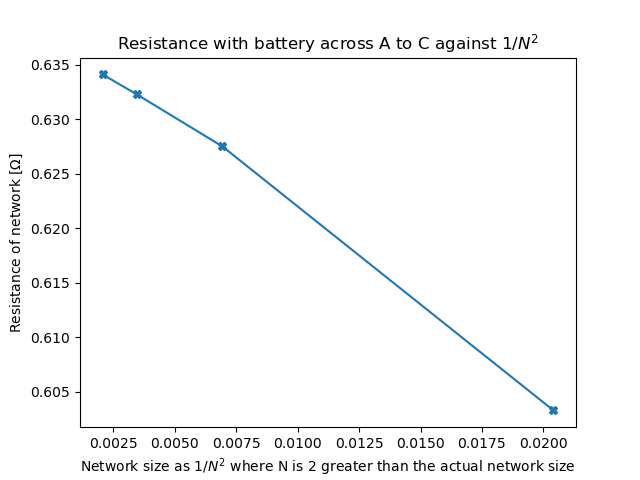
\includegraphics[scale=0.74]{./q7_2_AtoC.png} \\
    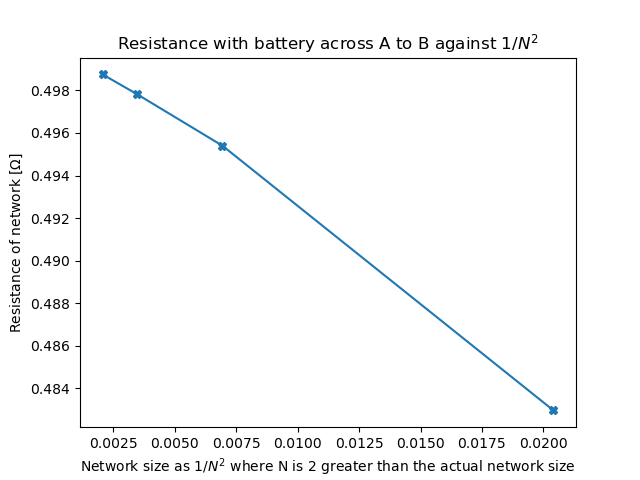
\includegraphics[scale=0.74]{./q7_2_AtoB.png} \\
    In order to estimate $N = \infty$ we can assume $1/N^{2} \rightarrow 0$, or in other
    words the y intecept. \\
    \begin{center}
        \begin{tabular}{|c||c|}
            \hline
            \multicolumn{2}{|c|}{Estimated values for $1/N^{2}$} \\
            \hline\hline
            A to C & \approx 0.635 \\
            A to B & \approx 0.5 \\
            \hline
        \end{tabular}
    \end{center}
    \section{q3}
    Here, we first simply need to modify our function for the new method. \\
    \lstinputlisting[language=Python, firstline=6, lastline=14]{./q7_3.py}
    In order to determine our new constant a, we can use a simple for loop to try many
    values of a and compare the new and the old results until they are very close to the same.
    \\
    Using a = 1 yields the follwing for network size 20x20 with battery connected from A to C:
    \begin{center}
        \begin{tabular}{|c|c|c|}
            \hline
            Algorithm used & Steps & Resistance [V] \\
            \hline\hline
            Old & 1295 & 0.6364830719829574 \\
            New & 114 & 0.633583420641185 \\
            \hline
        \end{tabular}
    \end{center}
    \\
    \lstinputlisting[language=Python, firstline=17]{./q7_3.py} \\
    This allows us to extract a value of a where the difference between the resistance of
    our new method and the resistance calculated by the old are extremely similar.
   \begin{center}
       $a \approx 1.70006$
   \end{center}
    Using this value of a fetches these results instead:
    \begin{center}
        \begin{tabular}{|c|c|c|}
            \hline
            Algorithm used & Steps & Resistance [V] \\
            \hline\hline
            New & 5 & 0.6362169192614182 \\
            \hline
        \end{tabular}
    \end{center}
    \\
    This value for resistance is much closer to using the old algorithm, but with only 5 steps,
    meaning it is roughly 259 times faster than using the old algorithm.
    \section{q4}
    In order to make measurements of the resistance between various pairs of points, we can modify the code
    like so.
    \lstinputlisting[language=Python, firstline=18]{./q7_4.py} \\
    Here, we set all of our nodes to measure from initially the same, and then depending on whether
    we want to measure horizontally or diagonally we increment accordingly.
    \\
    Plotting the increase in physical node separation vs resistance looks like so.
    \\
    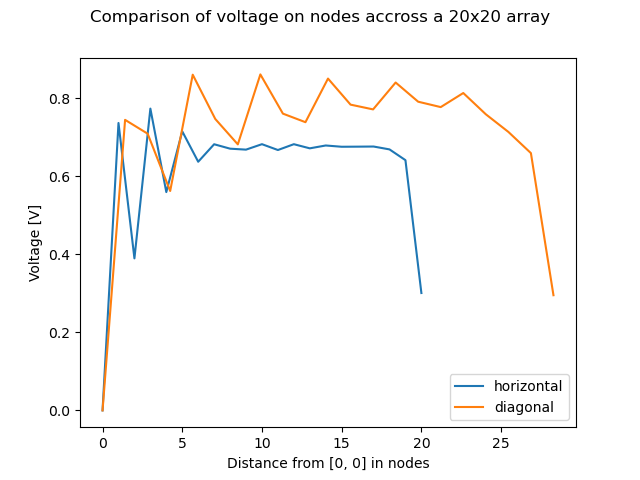
\includegraphics[scale=0.74]{./q7_4.png}
    \\
    Here we see a trend where, diagonal on average has higher resistace no matter the node 
    difference, but both trend toward a single value.\\
    We can see a sharp dip in both as N approaches 20 and $20\sqrt{2}$ for horizontal and diagonal
    respectively. This is likely due to the network running out of nodes to compare against.\\
    We can remedy this by setting our network size to something larger, say 25 but still only iterate
    over a node network of 20 nodes. \\
    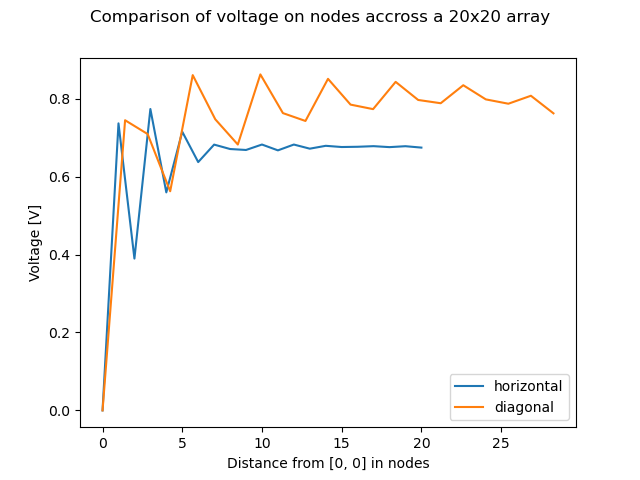
\includegraphics[scale=0.74]{./q7_4new.png}
\end{document}
